\documentclass[UTF8,a4paper,zihao=-4,fontset=none]{ctexart}

\usepackage[a4paper,left=3.17cm,right=3.17cm,top=2.54cm,bottom=2.54cm]{geometry}
\usepackage{fontspec}
\usepackage{graphicx}
\usepackage{float}
\usepackage{booktabs}
\usepackage{array}
\usepackage{longtable}
\usepackage{caption}
\usepackage{fancyhdr}
\usepackage{titlesec}
\usepackage{xcolor}
\usepackage{hyperref}
\usepackage{indentfirst}
\usepackage{enumitem}
\usepackage{url}
\usepackage{tikz}
\usepackage{listings}
\usetikzlibrary{arrows.meta,positioning,shapes.geometric}

\setmainfont{Times New Roman}
\setCJKmainfont{Noto Serif CJK SC}
\setCJKsansfont{Noto Sans CJK SC}
\setCJKmonofont{Noto Sans CJK SC}
\setCJKfamilyfont{zhsong}{Noto Serif CJK SC}
\setCJKfamilyfont{zhhei}{Noto Sans CJK SC}
\setCJKfamilyfont{zhfs}{Noto Serif CJK SC}
\setCJKfamilyfont{zhkai}{Noto Serif CJK SC}
\graphicspath{{figures/}{style/}}

\definecolor{cumtblue}{RGB}{0,56,132}
\definecolor{deepred}{RGB}{128,35,32}
\definecolor{textgray}{RGB}{48,48,48}
\definecolor{codebg}{RGB}{248,248,248}
\definecolor{codeframe}{RGB}{210,210,210}

\newcommand{\reporttitle}{基于 SAM 3.1 的开放词汇视频目标分割实验}

\hypersetup{
  unicode=true,
  colorlinks=true,
  linkcolor=black,
  citecolor=black,
  urlcolor=cumtblue,
  pdftitle={基于 SAM 3.1 的开放词汇视频目标分割实验},
  pdfauthor={卜炜珏}
}

\pagestyle{fancy}
\setlength{\headheight}{14.5pt}
\fancyhf{}
\fancyhead[C]{\small \reporttitle}
\fancyfoot[C]{\small \thepage}
\renewcommand{\headrulewidth}{0.4pt}
\renewcommand{\footrulewidth}{0pt}

\ctexset{
  section={
    format=\Large\bfseries\raggedright,
    name={第,章},
    number=\chinese{section},
    aftername=\quad
  },
  subsection={
    format=\large\bfseries\raggedright
  },
  subsubsection={
    format=\normalsize\bfseries\raggedright
  }
}

\captionsetup{font=small,labelfont=bf,labelsep=quad}
\setlength{\parindent}{2em}
\setlength{\parskip}{0pt}
\linespread{1.35}
\emergencystretch=3em
\Urlmuskip=0mu plus 2mu
\newcolumntype{L}[1]{>{\raggedright\arraybackslash}p{#1}}
\newcommand{\codepath}[1]{\path{#1}}
\setlist[itemize]{leftmargin=2.5em,itemsep=2pt,topsep=2pt}
\setlist[enumerate]{leftmargin=2.5em,itemsep=2pt,topsep=2pt}

\lstdefinestyle{pythoncode}{
  language=Python,
  basicstyle=\ttfamily\footnotesize,
  keywordstyle=\color{cumtblue}\bfseries,
  stringstyle=\color{deepred},
  commentstyle=\color{textgray},
  numbers=left,
  numberstyle=\scriptsize\color{textgray},
  stepnumber=1,
  numbersep=8pt,
  frame=single,
  rulecolor=\color{codeframe},
  backgroundcolor=\color{codebg},
  breaklines=true,
  columns=fullflexible,
  showstringspaces=false,
  tabsize=2
}

\lstdefinestyle{shellcode}{
  basicstyle=\ttfamily\footnotesize,
  keywordstyle=\color{cumtblue}\bfseries,
  stringstyle=\color{deepred},
  commentstyle=\color{textgray},
  numbers=left,
  numberstyle=\scriptsize\color{textgray},
  stepnumber=1,
  numbersep=8pt,
  frame=single,
  rulecolor=\color{codeframe},
  backgroundcolor=\color{codebg},
  breaklines=true,
  columns=fullflexible,
  showstringspaces=false,
  tabsize=2
}

\lstdefinestyle{jsoncode}{
  basicstyle=\ttfamily\footnotesize,
  numbers=left,
  numberstyle=\scriptsize\color{textgray},
  stepnumber=1,
  numbersep=8pt,
  frame=single,
  rulecolor=\color{codeframe},
  backgroundcolor=\color{codebg},
  breaklines=true,
  columns=fullflexible,
  showstringspaces=false,
  tabsize=2
}

\begin{document}

\begin{titlepage}
  \centering
  \vspace*{1.2cm}
  
\includegraphics[width=0.38\textwidth]{cumt_logo.pdf}

  \vspace{1.4cm}
  {\zihao{1}\bfseries 课程实验报告\par}
  \vspace{0.9cm}
  {\zihao{-2}\bfseries \makebox[\textwidth][c]{\reporttitle}\par}
  \vspace{0.5cm}
  {\zihao{-3}\color{textgray} 模型结构、核心代码、运行流程与多提示词实验分析\par}

  \vfill
  \begin{tabular}{>{\bfseries}p{4cm}p{8cm}}
    课程名称： & 图像处理与计算机视觉 \\
    任课教师： & 邵志文 \\
    学生姓名： & 卜炜珏 \\
    学号： & 08231338 \\
    班级： & 计科3班 \\
    完成日期： & 2026 年 6 月 \\
  \end{tabular}

  \vfill
  {\zihao{-4} 中国矿业大学\par}
\end{titlepage}

\pagenumbering{Roman}
\begin{abstract}
本次作业选用 Meta 官方开源的 SAM 3.1，在一段足球短视频上完成开放词汇目标分割与跨帧跟踪，并补充若干单帧图像提示实验。实验采用官方 SAM3 代码仓库，模型权重从 ModelScope 的 \texttt{facebook/sam3.1} 仓库下载，运行环境为 NVIDIA GeForce RTX 4090、Python 3.12 和 PyTorch 2.6.0+cu124。报告重点分析项目代码结构、PyTorch 模块构建、checkpoint 加载、推理上下文、Object Multiplex 张量映射、可视化输出流程和本地实验脚本，并使用 \texttt{person}、\texttt{ball}、\texttt{player in red} 三组视频文本提示词完成对比实验。实验结果显示，SAM 3.1 能根据自然语言提示发现不同粒度的目标实例，并在连续视频帧中保持较稳定的目标编号和分割结果；单帧实验进一步展示了场景级、物体级和部件级提示的输出差异。

\textbf{关键词：} SAM 3.1；开放词汇分割；视频目标跟踪；Object Multiplex；PyTorch
\end{abstract}

\clearpage
\tableofcontents
\clearpage

\pagenumbering{arabic}

\section{实验项目与研究背景}

\subsection{项目选择}

项目选用 Meta 的 SAM 3: Segment Anything with Concepts，它是 SAM 系列的第三代统一分割基础模型，也是本次课程作业中的图像处理深度学习开源项目。官方仓库位于 GitHub\cite{sam3_github}，项目页说明了模型定位并提供了示例演示\cite{sam3_project}。本次实验的脚本、报告和结果截图整理在个人公开仓库中\cite{homework_repo}，官方源码和模型权重不随作业仓库上传。SAM 3 支持文本、点、框、mask 等多种提示方式。相比 SAM 2，SAM 3 的关键变化是增加了开放词汇概念分割能力：用户输入简短文本短语后，模型可以自动检测并分割相关实例。

SAM 3.1 是 2026 年 3 月发布的更新版本，重点引入 Object Multiplex，用共享记忆方式联合处理多个视频目标，降低多目标跟踪中的重复计算\cite{sam3_release}。实验中直接加载 \texttt{sam3.1\_multiplex.pt} checkpoint，用文本提示词在足球视频帧序列中完成分割与跟踪。

\subsection{实验目标}

实验工作分为三块。工程部分是在本地 GPU 上配置独立 Conda 环境、下载权重并跑通 SAM 3.1 推理；代码部分从 PyTorch 源码角度梳理仓库结构、模型构建入口、\texttt{state\_dict} 加载、session 推理接口、Object Multiplex 张量映射、可视化工具和本地脚本改造；结果部分以视频目标分割为主，配合单帧图像提示实验，观察粗粒度类别、小目标、属性约束和部件级提示的输出差异。

\subsection{实验环境}

依赖安装在独立环境 \texttt{sam31} 中，没有写入 base 环境。由于本机 NVIDIA 驱动显示 CUDA 12.4，实验没有直接使用官方 README 中的 CUDA 12.8 PyTorch 命令，而是安装与当前驱动兼容的 PyTorch 2.6.0+cu124 预编译包\cite{pytorch_install}。环境配置见表~\ref{tab:env}。

\begin{table}[H]
  \centering
  \small
  \caption{实验运行环境}
  \label{tab:env}
  \begin{tabular}{L{4.2cm}L{8.2cm}}
    \toprule
    项目 & 配置 \\
    \midrule
    操作系统 & Linux \\
    Conda 环境 & \texttt{sam31} \\
    Python & 3.12.13 \\
    GPU & NVIDIA GeForce RTX 4090 \\
    GPU 显存 & 49140 MiB \\
    PyTorch & \texttt{2.6.0+cu124} \\
    TorchVision & \texttt{0.21.0+cu124} \\
    CUDA Runtime & 12.4 \\
    模型权重 & \texttt{sam3.1\_multiplex.pt}，来自 ModelScope\cite{modelscope_sam31} \\
    \bottomrule
  \end{tabular}
\end{table}

\section{SAM 3.1 项目代码结构解读}

\subsection{官方仓库结构}

官方仓库采用标准 Python 包结构。根目录提供说明文档、发布说明、包配置和示例资源，核心实现位于 \texttt{sam3/} 包内。主要目录见表~\ref{tab:repo-structure}。

\begin{longtable}{L{4.1cm}L{9.0cm}}
  \caption{SAM3 官方仓库结构说明}
  \label{tab:repo-structure} \\
  \toprule
  路径 & 作用 \\
  \midrule
  \endfirsthead
  \toprule
  路径 & 作用 \\
  \midrule
  \endhead
  \codepath{README.md} & 项目介绍、环境安装、基础图像和视频推理示例。 \\
  \codepath{RELEASE_SAM3p1.md} & SAM 3.1 发布说明，介绍 Object Multiplex、效率提升和新 checkpoint。 \\
  \codepath{pyproject.toml} & Python 包配置和基础依赖。 \\
  \codepath{examples/} & 官方 notebook 示例，包括图像预测、视频预测、批量推理和 SAM 3.1 multiplex 示例。 \\
  \codepath{assets/} & 官方示例图片、GIF、模型结构图和效率图。 \\
  \codepath{sam3/model_builder.py} & 模型构建入口，封装图像模型、视频模型和 SAM 3.1 multiplex predictor。 \\
  \codepath{sam3/model/} & 核心模型模块，包括编码器、检测器、跟踪器、multiplex 跟踪和 session predictor。 \\
  \codepath{sam3/sam/} & SAM 系列基础模块，包括 prompt encoder、mask decoder 和 Transformer。 \\
  \codepath{sam3/visualization_utils.py} & 将分割 mask、边界框和目标编号绘制到原始图像上的工具。 \\
  \codepath{scripts/eval/} & benchmark 评估、数据下载和格式转换脚本。 \\
  \bottomrule
\end{longtable}

\subsection{模型结构}

SAM 3 由 detector 和 tracker 组成，二者共享视觉编码器。detector 负责根据文本、几何提示和图像特征发现目标实例，tracker 负责在视频帧之间传播目标记忆并输出连续的 masklet。官方结构如图~\ref{fig:sam3-model} 所示。

\begin{figure}[H]
  \centering
  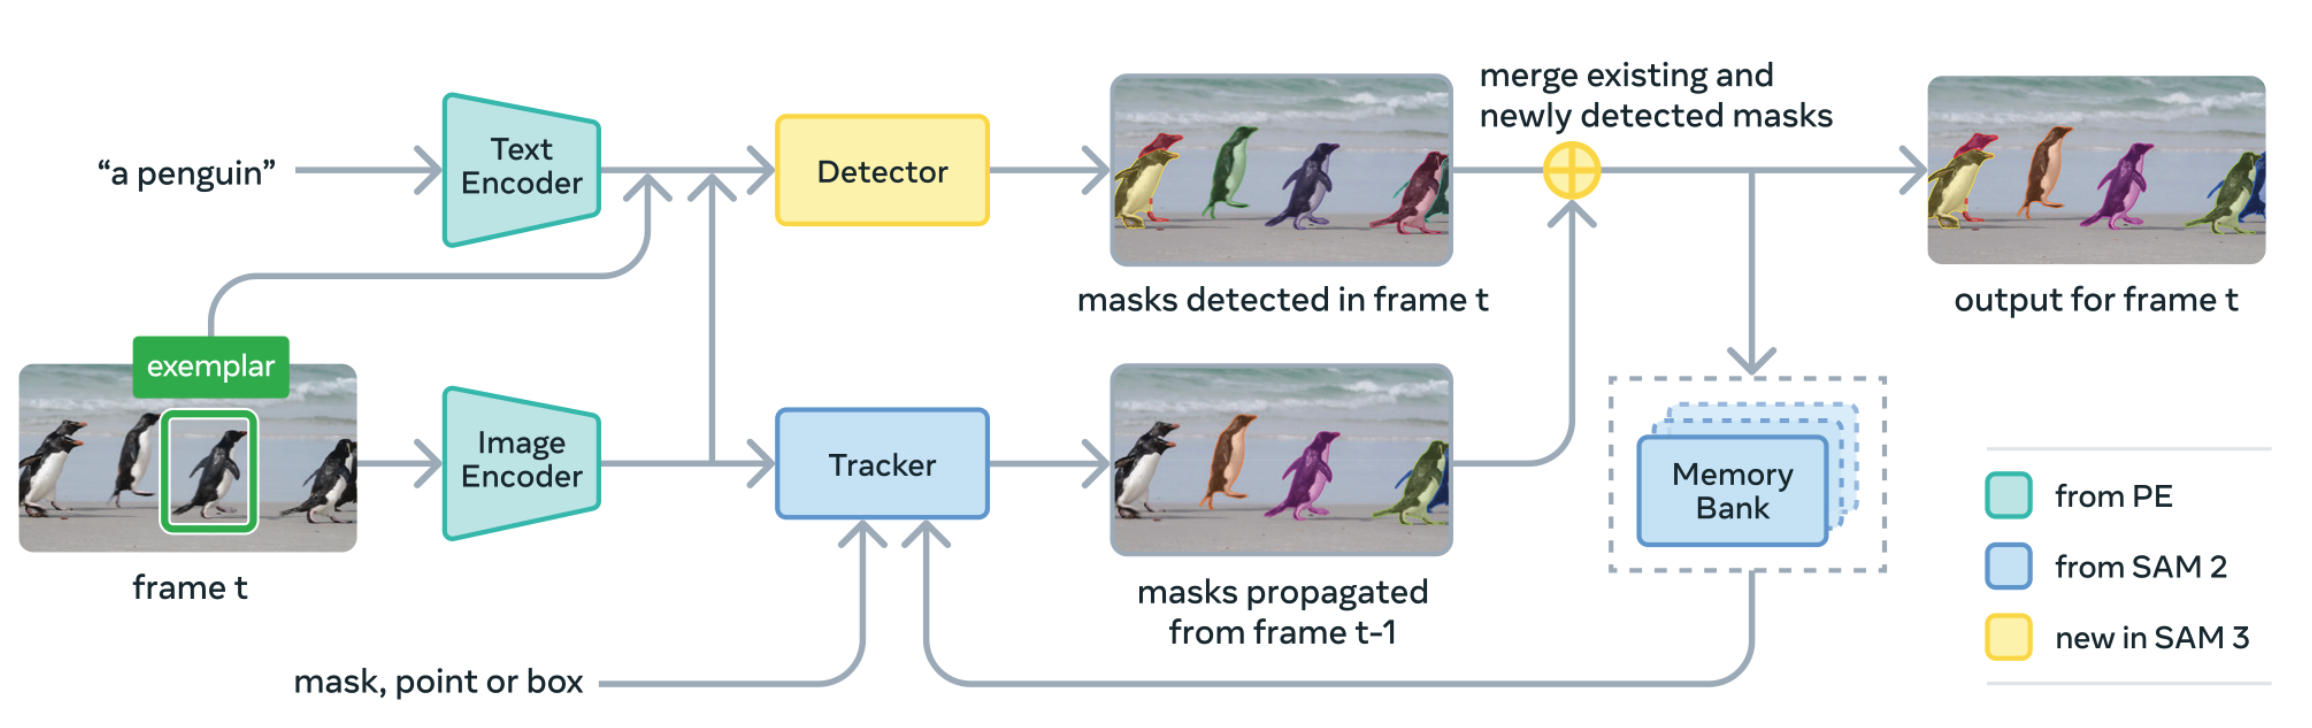
\includegraphics[width=0.92\textwidth]{sam3-model-diagram.png}
  \caption{SAM 3 官方模型结构图。模型将视觉特征、文本提示和几何提示融合，用 detector 输出实例，再由 tracker 完成视频传播。}
  \label{fig:sam3-model}
\end{figure}

SAM 3.1 的 Object Multiplex 主要针对视频跟踪阶段。原始 SAM 3 对每个目标相对独立地处理记忆，目标数增加时容易产生重复计算；SAM 3.1 将多个对象组织到固定容量的 bucket 中联合传播，减少记忆读取与更新的重复开销。图~\ref{fig:sam31-multiplex} 展示了官方的 multiplex 思路。

\begin{figure}[H]
  \centering
  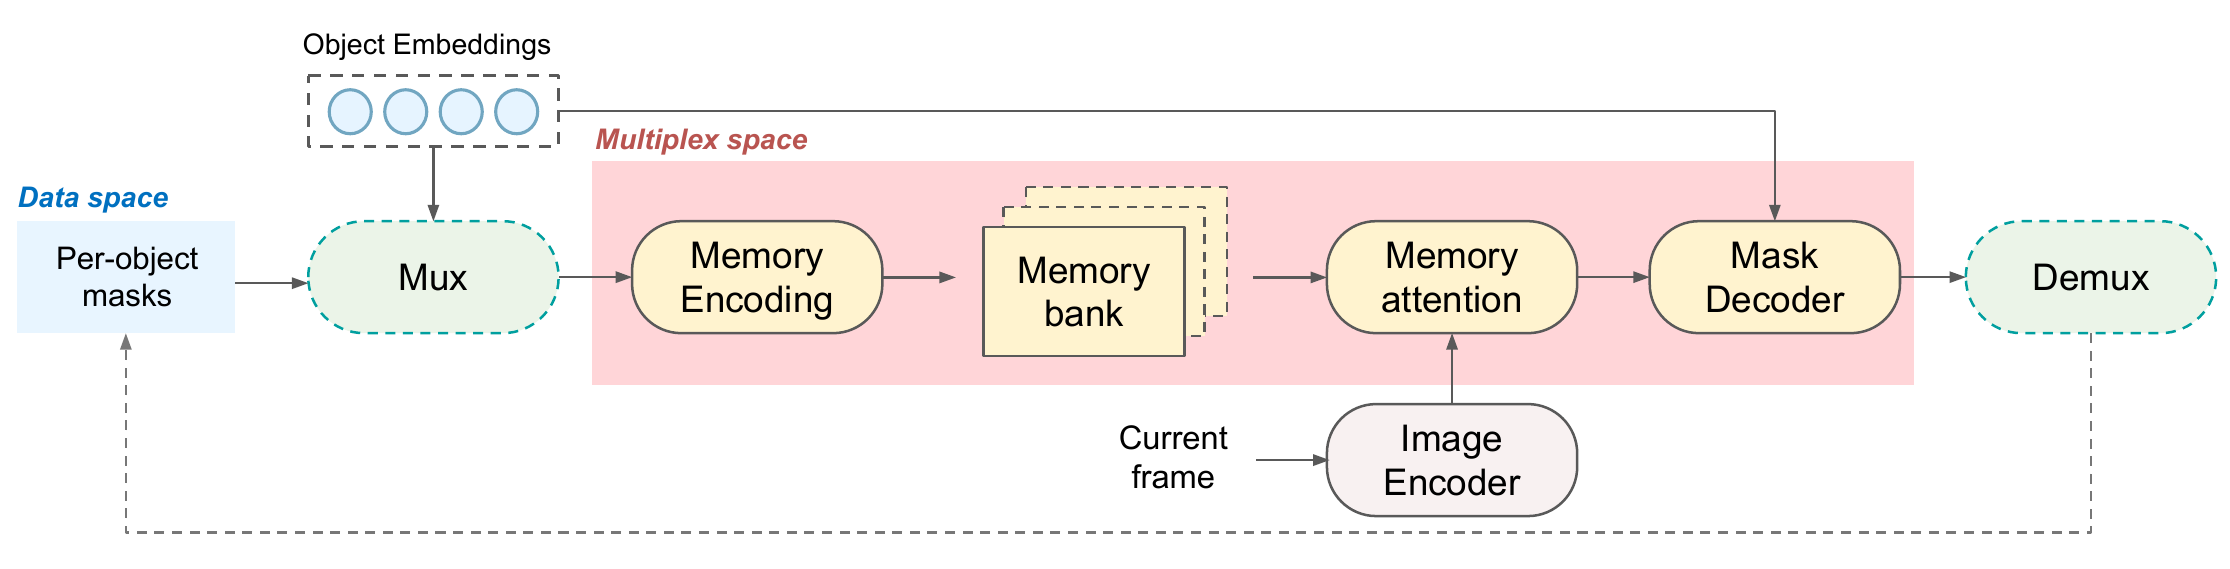
\includegraphics[width=0.88\textwidth]{sam31-multiplex-diagram.png}
  \caption{SAM 3.1 Object Multiplex 示意图。多个对象共享一组记忆处理流程，以提高多目标视频跟踪效率。}
  \label{fig:sam31-multiplex}
\end{figure}

\section{核心代码分析}

\subsection{官方 PyTorch 源码调用链概览}

SAM 3.1 的视频推理由模型构建、请求分发、交互式跟踪和 multiplex 张量转换四个模块依次协作完成，不存在一个函数包揽全部逻辑的入口。表~\ref{tab:source-chain} 按实验实际执行顺序整理了主要源码位置。报告中的本地脚本只负责抽帧、传参和保存结果，核心 detector、tracker、session、Object Multiplex 和 PyTorch 张量计算逻辑均来自官方仓库。

\begin{table}[H]
  \centering
  \scriptsize
  \setlength{\tabcolsep}{2.5pt}
  \caption{SAM 3.1 视频推理源码调用链}
  \label{tab:source-chain}
  \begin{tabular}{L{3.0cm}L{5.6cm}L{4.5cm}}
    \toprule
    源码位置 & 关键类或函数 & 在实验中的作用 \\
    \midrule
    \codepath{sam3/model_builder.py} & \texttt{build\_sam3\_multiplex\_video\_predictor} & 组装多个 \texttt{nn.Module} 子模块，加载 checkpoint，并返回统一 predictor。 \\
    \codepath{sam3/model/sam3_base_predictor.py} & \texttt{Sam3BasePredictor} & 提供 \texttt{handle\_request} 和 \texttt{handle\_stream\_request}，把外部请求转发给底层模型。 \\
    \codepath{sam3/model/sam3_multiplex_video_predictor.py} & \texttt{Sam3MultiplexVideoPredictor} & 保存 session 参数、默认阈值和异步加载配置，是视频实验直接使用的 predictor 类型。 \\
    \codepath{sam3/model/sam3_multiplex_tracking.py} & \texttt{Sam3MultiplexTrackingWithInteractivity} & 处理文本、点、框等交互提示，并决定全量传播、局部传播或读取缓存结果。 \\
    \codepath{sam3/model/multiplex_utils.py} & \texttt{MultiplexState}、\texttt{MultiplexController} & 维护 object 到 bucket/slot 的映射，用 PyTorch 矩阵乘法实现 \texttt{mux} 和 \texttt{demux}。 \\
    \codepath{sam3/model/video_tracking_multiplex.py} & \texttt{VideoTrackingDynamicMultiplex} 相关方法 & 在 mask decoder、memory encoder 和 object pointer 更新中实际执行张量 reshape、拼接、索引和矩阵映射。 \\
    \bottomrule
  \end{tabular}
\end{table}

从实验角度看，关注点并不在于某层网络的全部参数，而是这些 PyTorch 模块如何把文本提示逐步转化为跨帧 mask 输出。后续分析因此围绕 \texttt{nn.Module} 组装、\texttt{state\_dict} 加载、推理上下文、张量 shape 变化和后处理输出展开。

\subsection{模型构建入口}

模型构建的入口位于 \codepath{sam3/model_builder.py}，核心函数是 \codepath{build_sam3_multiplex_video_predictor}。从 PyTorch 角度看，这个函数的主要工作是把 detector、tracker、text encoder、mask decoder 等多个 \texttt{nn.Module} 子模块拼成一个可推理的组合模型，再把 checkpoint 中的权重张量加载到对应模块。

\begin{lstlisting}[style=pythoncode,caption={SAM 3.1 multiplex predictor 构建示例}]
from sam3.model_builder import build_sam3_multiplex_video_predictor

predictor = build_sam3_multiplex_video_predictor(
    checkpoint_path="checkpoints/sam3.1/sam3.1_multiplex.pt",
    use_fa3=False,
    compile=False,
    warm_up=False,
    async_loading_frames=False,
)
\end{lstlisting}

构建函数先创建底层的 multiplex video model，再将 tracker 自身的 backbone 置空并交由交互式模型统一管理，最后通过 \texttt{Sam3MultiplexPredictorWrapper} 标记为 multiplex 动态模式。这样做的目的是避免 tracker 和 demo model 各维护一份独立的 backbone。随后，代码创建 detector 侧的 \texttt{SAM3VLBackboneTri}、transformer、segmentation head、geometry encoder 和 scoring 模块，并把它们作为子模块传入 \texttt{Sam3MultiplexDetector}。

构建函数最后把 detector 与 tracker 包装进交互式 tracking 模块，并设置检测阈值、NMS 阈值、关联 IoU 阈值、新目标阈值、热启动参数、重建参数和 \texttt{max\_num\_objects}。因此，\codepath{build_sam3_multiplex_video_predictor} 并不只是读一个权重文件，而是把开放词汇检测和视频跟踪两条 PyTorch 计算路径装配成一个可交互系统。

\begin{lstlisting}[style=pythoncode,caption={模型构建与 checkpoint 键名映射的源码逻辑摘录}]
tracker_model = build_sam3_multiplex_video_model(...)
del tracker_model.backbone
tracker_model.backbone = None

tracker = Sam3MultiplexPredictorWrapper(
    model=tracker_model,
    is_multiplex=True,
    is_multiplex_dynamic=True,
)
detector = Sam3MultiplexDetector(...)
demo_model = Sam3MultiplexTrackingWithInteractivity(
    tracker=tracker,
    detector=detector,
    max_num_objects=max_num_objects,
    recondition_every_nth_frame=16,
)

ckpt = torch.load(checkpoint_path, map_location="cpu", weights_only=True)
needs_remap = any(
    k.startswith("sam3_model.") or k.startswith("sam2_predictor.") for k in ckpt
)
if needs_remap:
    remapped_ckpt = {}
    for k, v in ckpt.items():
        if k.startswith("sam3_model."):
            k = "detector." + k[len("sam3_model."):]
        elif k.startswith("sam2_predictor."):
            k = "tracker." + k[len("sam2_predictor."):]
        remapped_ckpt[k] = v
    ckpt = remapped_ckpt
demo_model.load_state_dict(ckpt, strict=False)
predictor = Sam3MultiplexVideoPredictor(model=demo_model, ...)
\end{lstlisting}

源码先调用 \codepath{torch.load(..., map_location="cpu", weights_only=True)}，将 checkpoint 读到 CPU，避免一开始就占用 GPU 显存。随后使用 \codepath{load_state_dict(strict=False)} 将权重映射到 \texttt{demo\_model}。这里的 \texttt{strict=False} 允许加载过程返回 \texttt{missing\_keys} 和 \texttt{unexpected\_keys}，便于兼容旧命名或不同发布格式，但不会绕过形状不匹配。最后的 \codepath{demo_model.cuda().eval()} 是标准 PyTorch 推理设置：模型参数移入 GPU，并把 BatchNorm、Dropout 等模块切到评估模式。

实验关闭了 \texttt{use\_fa3}，因为 FlashAttention 3 是可选加速组件，不参与正确性验证。\texttt{max\_num\_objects} 和 \texttt{multiplex\_count} 均使用默认值 16，与官方 checkpoint 参数形状匹配；若手动改为 8，加载时 checkpoint 中对应权重的维度与模型定义不一致，无法通过 \texttt{load\_state\_dict} 检查。

\subsection{PyTorch 推理上下文与混合精度}

SAM3.1 的推理路径显式使用了 PyTorch 的推理上下文和混合精度机制。请求分发函数 \texttt{handle\_request} 与 \texttt{handle\_stream\_request} 均带有 \texttt{@torch.inference\_mode()} 装饰器，交互式 tracking 的 \texttt{init\_state}、\texttt{add\_prompt}、\texttt{propagate\_in\_video} 也使用同类装饰。按照 PyTorch 文档\cite{pytorch_api_docs}，\texttt{inference\_mode} 会关闭梯度追踪和 autograd 相关状态，减少推理阶段不必要的内存记录。

\begin{lstlisting}[style=pythoncode,caption={推理上下文与混合精度相关源码摘录}]
class Sam3MultiplexVideoPredictor(Sam3BasePredictor):
    def __init__(self, model, ...):
        self.model = model
        torch.backends.cuda.matmul.allow_tf32 = True
        torch.backends.cudnn.allow_tf32 = True
        self.bf16_context = torch.autocast(
            device_type="cuda",
            dtype=torch.bfloat16,
        )
        self.bf16_context.__enter__()

@torch.inference_mode()
def handle_request(self, request):
    ...

with torch.autocast(device_type="cuda", dtype=torch.bfloat16):
    frame_idx, outputs = self.model.add_prompt(**filtered_kwargs)
\end{lstlisting}

这段源码说明官方实现不是在普通 Python 函数里直接跑网络，而是在 PyTorch 推理环境下执行：TF32 被允许用于 Ampere 架构 GPU 的矩阵乘法和 cuDNN 计算，\texttt{torch.autocast(device\_type="cuda", dtype=torch.bfloat16)} 则让合适的 CUDA 算子自动使用 bfloat16。对本实验的 RTX 4090 来说，这可以降低显存压力并提高吞吐；同时，由于最后输出会转为 mask、box 和 score，这些推理优化不改变脚本对外拿到的数据结构。

\subsection{Session 式视频推理}

SAM3 视频 predictor 采用请求分发接口。外部调用不直接访问底层模型，而是向 predictor 发送带有 \texttt{type} 字段的请求。请求分发逻辑位于 \codepath{sam3/model/sam3_base_predictor.py}，常用请求包括 \texttt{start\_session}、\texttt{add\_prompt}、\texttt{propagate\_in\_video} 和 \texttt{close\_session}。

\begin{lstlisting}[style=pythoncode,caption={文本提示和跨帧传播的核心调用}]
response = predictor.handle_request(
    request={
        "type": "add_prompt",
        "session_id": session_id,
        "frame_index": 0,
        "text": "person",
    }
)

outputs_per_frame = {0: response["outputs"]}
for response in predictor.handle_stream_request(
    request={
        "type": "propagate_in_video",
        "session_id": session_id,
    }
):
    outputs_per_frame[response["frame_index"]] = response["outputs"]
\end{lstlisting}

这种设计把交互式分割建模为有状态的会话：session 初始化时一次性加载帧序列，之后可以在任意帧上追加文本、点或框提示，再触发视频范围的传播，无需重复加载图像或重建模型状态。源码中 \texttt{Sam3BasePredictor.start\_session} 会调用底层模型的 \texttt{init\_state}，并把返回的 \texttt{inference\_state} 存入 \texttt{\_all\_inference\_states}。后续每次请求都通过 \texttt{session\_id} 找回这份状态，因此视频帧缓存、目标 id、用户提示历史和 tracker metadata 可以在多轮交互之间保留下来。

\begin{lstlisting}[style=pythoncode,caption={请求分发与参数过滤的源码逻辑摘录}]
def handle_request(self, request):
    if request["type"] == "add_prompt":
        return self.add_prompt(
            session_id=request["session_id"],
            frame_idx=request["frame_index"],
            text=request.get("text"),
            points=request.get("points"),
            bounding_boxes=request.get("bounding_boxes"),
        )

def add_prompt(self, session_id, frame_idx, text=None, **kwargs):
    session = self._get_session(session_id)
    inference_state = session["state"]
    call_args = {
        "inference_state": inference_state,
        "frame_idx": frame_idx,
        "text_str": text,
        **kwargs,
    }
    sig = inspect.signature(self.model.add_prompt)
    valid_params = set(sig.parameters.keys())
    call_args = {k: v for k, v in call_args.items() if k in valid_params}
    frame_idx, outputs = self.model.add_prompt(**call_args)
    return {"frame_index": frame_idx, "outputs": outputs}
\end{lstlisting}

基类通过 \texttt{inspect.signature} 自动过滤不支持的参数，使同一套 \texttt{handle\_request} 可以兼容 SAM3 与 SAM3.1 之间签名略有差异的底层方法。本地实验脚本中只构造统一的 request 字典即可工作，原因正在于此。

\subsection{交互式 tracking 源码流程}

真正处理 SAM 3.1 视频交互的是 \texttt{sam3\_multiplex\_tracking.py} 中的交互式 tracking 类。它继承自 \texttt{Sam3MultiplexTracking}，在基础视频 grounding 上增加了用户行为记录、局部细化和缓存读取逻辑。初始化时，\texttt{init\_state} 会在基础状态中加入 \texttt{action\_history}；如果 tracker 处于 per-object 模式，还会初始化内部 SAM2-style 跟踪状态。本实验使用的是 multiplex 动态模式，因此多目标状态主要由 tracker metadata 和 multiplex state 管理。

\texttt{add\_prompt} 会根据提示类型走两条路径：如果输入点提示，则调用 \texttt{add\_sam2\_new\_points} 对已有目标做局部细化；如果输入文本或框提示，则临时关闭 \texttt{use\_batched\_grounding}，再调用父类的 SAM3 grounding 流程。文本提示关闭 batched grounding，是因为这一分支主要依赖 detector 的开放词汇检测结果；点提示通常用于已有目标的局部修正，更接近 SAM2 风格的 per-object 细化。实验中的 \texttt{person}、\texttt{ball} 和 \texttt{player in red} 都属于文本提示，流程是 detector 根据文本生成候选目标，后处理得到初始 mask 和 object id，再把这些目标写入视频状态。

\texttt{propagate\_in\_video} 在传播前会读取 \texttt{action\_history}，判断当前应执行全量 video grounding、局部 SAM2 传播，还是直接返回已有缓存。首次文本提示后通常进入全量传播路径；如果后续用户只用点提示修正某个对象，则源码可以只传播被修正的目标，并与已有 video grounding 结果合并。全量传播内部会继续调用 \texttt{video\_tracking\_multiplex.py} 中的 mask decoder 和 memory encoder，此时 multiplex state 负责完成 bucket 与目标索引之间的张量转换。本实验走的是文本提示后的全量路径，即一次 grounding 后传播到每一帧。

\subsection{输出数据结构与 PyTorch 后处理}

每帧返回的输出字典包含四个核心字段，见表~\ref{tab:output-fields}。\texttt{out\_obj\_ids} 为每个目标分配编号，\texttt{out\_binary\_masks} 和 \texttt{out\_boxes\_xywh} 分别给出分割区域和归一化边界框，\texttt{out\_probs} 则提供置信度，用于按阈值筛选或排序。

\begin{table}[H]
  \centering
  \small
  \caption{SAM 3.1 视频输出字段}
  \label{tab:output-fields}
  \begin{tabular}{L{4.1cm}L{4.0cm}L{5.0cm}}
    \toprule
    字段 & 含义 & 后续用途 \\
    \midrule
    \texttt{out\_binary\_masks} & 每个实例对应的二值分割 mask & 叠加到原始帧形成可视化结果。 \\
    \texttt{out\_boxes\_xywh} & 归一化边界框，格式为 x、y、w、h & 绘制目标框，辅助观察目标位置。 \\
    \texttt{out\_probs} & 每个实例的置信度 & 在图上显示 score，帮助判断输出可靠性。 \\
    \texttt{out\_obj\_ids} & 跟踪目标编号 & 观察同一对象在不同帧中的 id 是否稳定。 \\
    \bottomrule
  \end{tabular}
\end{table}

这些字段来自 \texttt{Sam3MultiplexTracking.\_postprocess\_output} 的 PyTorch 后处理。源码先从 \texttt{obj\_id\_to\_mask} 字典中取出目标 id，并使用 \texttt{torch.tensor}、\texttt{torch.cat} 将分散的 mask 合并为形状为 $N \times H \times W$ 的布尔张量，其中 $N$ 是当前帧保留的目标数。随后用 \texttt{out\_binary\_masks.any(dim=(1, 2))} 删除面积为 0 的 mask；如存在被抑制或删除的目标，再用 \texttt{torch.isin}、\texttt{torch.nonzero} 和 \texttt{torch.index\_select} 做索引筛选。

\begin{lstlisting}[style=pythoncode,caption={输出后处理中的 PyTorch 张量操作摘录}]
out_obj_ids = torch.tensor(curr_obj_ids, dtype=torch.int64)
out_binary_masks = torch.cat(
    [obj_id_to_mask[obj_id] for obj_id in curr_obj_ids],
    dim=0,
)
keep = out_binary_masks.any(dim=(1, 2)).cpu()
keep_idx = torch.nonzero(keep, as_tuple=True)[0]
keep_idx_gpu = keep_idx.pin_memory().to(
    device=out_binary_masks.device,
    non_blocking=True,
)
out_binary_masks = torch.index_select(out_binary_masks, 0, keep_idx_gpu)
out_boxes_xywh = box_xyxy_to_xywh(masks_to_boxes(out_binary_masks))
outputs = {
    "out_obj_ids": out_obj_ids.cpu().numpy(),
    "out_boxes_xywh": out_boxes_xywh.cpu().numpy(),
    "out_binary_masks": out_binary_masks.cpu().numpy(),
}
\end{lstlisting}

这里能看到从 GPU 张量到报告可视化数据的完整转换：mask 的筛选和 box 计算在 PyTorch 张量上完成，最终通过 \texttt{.cpu().numpy()} 转成 NumPy 数组，交给可视化函数绘图。边界框先以像素坐标计算，再除以视频宽高归一化，因此表中 \texttt{out\_boxes\_xywh} 的数值可直接用于不同分辨率图像上的显示。

\subsection{Object Multiplex 跟踪逻辑}

Multiplex 状态管理位于 \texttt{multiplex\_utils.py}。其中 \texttt{MultiplexController} 继承自 \texttt{nn.Module}，负责根据目标数和 \texttt{multiplex\_count} 计算 bucket 数；\texttt{MultiplexState} 保存二维 \texttt{assignments}，外层是 bucket，内层是 bucket 中的 slot。普通目标使用非负索引，空 slot 用 \texttt{-1} 表示，被删除目标用 \texttt{-1116} 标记。这样，模型可以把任意数量的目标补齐到 \texttt{num\_buckets} $\times$ \texttt{multiplex\_count} 的规则形状。

\begin{lstlisting}[style=pythoncode,caption={MultiplexState 中 mux 和 demux 的简化逻辑}]
class MultiplexState:
    def _precompute_transition_matrices(self):
        mux_matrix = zeros(num_buckets * multiplex_count, total_valid_entries)
        demux_matrix = zeros(total_valid_entries, num_buckets * multiplex_count)
        for bucket_id, bucket in enumerate(assignments):
            for slot_id, object_idx in enumerate(bucket):
                if object_idx >= 0:
                    flat_slot = bucket_id * multiplex_count + slot_id
                    mux_matrix[flat_slot, object_idx] = 1.0
                    demux_matrix[object_idx, flat_slot] = 1.0

    def mux(self, x):
        # data space: [num_objects, ...]
        # multiplex space: [num_buckets, multiplex_count, ...]
        return (self.mux_matrix @ flatten(x)).view(mux_shape)

    def demux(self, x):
        # multiplex space -> data space, padding slots are ignored
        return (self.demux_matrix @ flatten(x)).view(data_shape)
\end{lstlisting}

源码的核心是两张预计算的 PyTorch 矩阵：\texttt{mux\_matrix} 的形状为 $(B \times M) \times N$，\texttt{demux\_matrix} 的形状为 $N \times (B \times M)$，其中 $B$ 是 bucket 数，$M$ 是 \texttt{multiplex\_count}，$N$ 是有效目标数。\texttt{mux} 先把输入张量 reshape 成 $N \times F$，再执行 \texttt{self.mux\_matrix @ x\_flat}，最后 view 成 $B \times M \times \cdots$；\texttt{demux} 则执行相反方向的矩阵乘法。由于 padding slot 在矩阵中没有有效映射，空位不会进入最终实例列表。

实际张量转换分布在 \texttt{video\_tracking\_multiplex.py}。在 mask decoder 的 propagation 分支中，\texttt{sam\_mask\_decoder} 输出的 \texttt{low\_res\_multimasks}、\texttt{ious}、\texttt{object\_score\_logits} 和 \texttt{sam\_output\_tokens} 先处在 $B \times M$ 的 multiplex 空间，随后统一调用 \texttt{multiplex\_state.demux(...)} 还原为 $N$ 个目标。记忆写入路径则相反：\texttt{\_encode\_new\_memory} 中的 \texttt{mask\_for\_mem} 先通过 \texttt{multiplex\_state.mux(...)} 转成 bucket 形式，再送入 \texttt{maskmem\_backbone}。

新增目标时，\texttt{add\_new\_masks\_to\_existing\_state} 还要更新 bucket/slot 分配。源码首先将已有目标的 \texttt{obj\_ptr} 从 multiplex 空间 \texttt{demux} 到数据空间，附加新目标的 pointer 张量，再通过 \texttt{torch.cat} 合并为新的 pointer 序列，最后用 \texttt{multiplex\_state.mux(combined\_pointers)} 写回状态。旧目标本身没有变化，但它们在 bucket 中的位置可能因动态重分配而变化，这也是 multiplex controller 需要维护可逆映射的原因。

综上，Object Multiplex 的核心机制是在目标索引、bucket slot、object pointer 和 mask memory 之间维持一组可逆的线性映射矩阵，而不是简单地将多个 mask 拼成 batch。对外接口仍然返回按目标排列的 \texttt{out\_obj\_ids} 等字段，对内则通过 bucket 结构复用 memory encoder/decoder 的中间结果，避免随目标数线性增长的重复操作。

\subsection{可视化流程}

可视化函数位于 \codepath{sam3/visualization_utils.py}。本实验使用 \texttt{save\_masklet\_image} 将每帧输出保存为图片。该函数内部先读取原始帧，再调用渲染函数叠加 mask、边界框、object id 和置信度。

\begin{lstlisting}[style=pythoncode,caption={单帧可视化保存示例}]
save_masklet_image(
    frame=str(frames[frame_idx]),
    outputs=outputs_per_frame[frame_idx],
    out_path=str(output_path),
    alpha=0.5,
    frame_idx=frame_idx,
)
\end{lstlisting}

\subsection{本地实验脚本}

本地脚本 \texttt{scripts/run\_sam31\_player.py} 把官方 notebook 中的推理逻辑抽出来，改成命令行可复现的实验。该脚本不修改任何官方源码，独立完成 GIF 帧抽取、模型加载、session 创建、提示传播和结果保存五个环节，流程图见图~\ref{fig:pipeline}。

\begin{figure}[H]
  \centering
  \resizebox{0.96\textwidth}{!}{%
  \begin{tikzpicture}[
    box/.style={rectangle,rounded corners=4pt,draw=cumtblue,thick,fill=blue!5,minimum width=2.45cm,minimum height=1.05cm,align=center,font=\small},
    key/.style={rectangle,rounded corners=4pt,draw=deepred,thick,fill=red!5,minimum width=2.65cm,minimum height=1.05cm,align=center,font=\small},
    arrow/.style={-{Stealth[length=3mm]},thick,draw=textgray}
  ]
    \node[box] (gif) at (0,0) {读取\\player.gif};
    \node[box] (frames) at (3,0) {抽取\\JPEG 帧};
    \node[key] (model) at (6,0) {加载\\SAM 3.1};
    \node[key] (prompt) at (9,0) {添加\\文本提示};
    \node[box] (prop) at (12,0) {跨帧\\传播};
    \node[box] (vis) at (15,0) {保存\\截图与元数据};
    \draw[arrow] (gif) -- (frames);
    \draw[arrow] (frames) -- (model);
    \draw[arrow] (model) -- (prompt);
    \draw[arrow] (prompt) -- (prop);
    \draw[arrow] (prop) -- (vis);
  \end{tikzpicture}}
  \caption{本地实验脚本推理流程。脚本将视频帧抽取、模型加载、文本提示、跨帧传播和结果保存组织为可重复命令。}
  \label{fig:pipeline}
\end{figure}

脚本还增加了 \texttt{--output-prefix} 参数，避免不同提示词实验的图片、metadata 和日志相互覆盖。例如 \texttt{person} 对应 \texttt{sam31\_player\_person\_summary.png}，\texttt{ball} 对应 \texttt{sam31\_player\_ball\_summary.png}。

\begin{lstlisting}[style=pythoncode,caption={多提示词输出命名逻辑}]
parser.add_argument("--prompt", default="person", help="Text prompt.")
parser.add_argument(
    "--output-prefix",
    default=None,
    help="Output filename prefix. Defaults to a prompt-based slug.",
)

def slugify_prompt(prompt: str) -> str:
    slug = re.sub(r"[^a-z0-9]+", "_", prompt.lower()).strip("_")
    return slug or "prompt"

output_prefix = args.output_prefix or f"sam31_player_{slugify_prompt(args.prompt)}"
summary_path = args.results_dir / f"{output_prefix}_summary.png"
metadata_path = args.results_dir / f"{output_prefix}_metadata.json"
\end{lstlisting}

通过 \texttt{--output-prefix} 和 \texttt{slugify\_prompt}，不同 prompt 的输出文件会自动携带对应的前缀标识，避免相互覆盖。

脚本中还加入了 \texttt{start\_multiplex\_session} 辅助函数，直接调用 \texttt{predictor.model.init\_state} 并手动登记 session。这是为了适配当前 SAM3.1 multiplex 模型的参数签名：官方基类 \texttt{start\_session} 会传入 \texttt{offload\_state\_to\_cpu}，而本地安装版本的 multiplex \texttt{init\_state} 并不接收这个参数。该兼容逻辑只放在实验脚本中，不改官方源码，便于后续更新 SAM3 仓库时直接替换上游代码。

\subsection{单帧图像实验脚本}

除了视频 predictor，本实验还补充了 \texttt{scripts/run\_sam31\_image\_cases.py}。该脚本使用 \codepath{sam3/model/sam3_image_processor.py} 中的 \texttt{Sam3Processor}，在若干静态图片上执行文本提示分割。其核心调用更接近普通图像分割任务：先构建图像模型，再设置输入图像，最后输入文本 prompt 得到 masks、boxes 和 scores。

\begin{lstlisting}[style=pythoncode,caption={单帧图像文本提示调用}]
model = build_sam3_image_model(
    checkpoint_path=str(args.checkpoint),
    load_from_HF=False,
    compile=False,
)
processor = Sam3Processor(
    model,
    confidence_threshold=args.confidence_threshold,
)

state = processor.set_image(image)
output = processor.set_text_prompt(state=state, prompt=case.prompt)
\end{lstlisting}

该脚本用于补充 SAM 3.1 在静态图像上的开放词汇分割表现。实验选取了 \texttt{building}、\texttt{truck}、\texttt{wheel} 等成功样例，以及 \texttt{tree} 和 \texttt{bottle} 在默认阈值下未保留实例的对照样例，以展示不同提示词粒度和阈值设置对输出结果的影响。

\section{实验环境与运行流程}

\subsection{环境配置命令}

以下是环境搭建用到的关键命令。安装前确认当前 shell 位于 base 环境，但所有依赖均通过 \texttt{conda run -n sam31} 安装到独立环境。

\begin{lstlisting}[style=shellcode,caption={环境配置命令摘录}]
conda create -n sam31 python=3.12 -y

conda run -n sam31 python -m pip install \
    torch==2.6.0 torchvision==0.21.0 \
    --index-url https://download.pytorch.org/whl/cu124

conda run -n sam31 python -m pip install -e . \
    modelscope matplotlib opencv-python-headless imageio

conda run -n sam31 python -m pip install \
    einops pycocotools psutil pandas scikit-image scikit-learn
\end{lstlisting}

由于 SAM3 要求 \texttt{numpy<2}，且源码仍使用 \texttt{pkg\_resources}，实验中固定了两个兼容依赖：

\begin{lstlisting}[style=shellcode,caption={兼容依赖固定}]
conda run -n sam31 python -m pip install \
    --force-reinstall --no-deps numpy==1.26.4
conda run -n sam31 python -m pip install "setuptools<81"
\end{lstlisting}

\subsection{权重下载}

SAM 3.1 checkpoint 从 ModelScope 下载，避免 Hugging Face gated checkpoint 登录问题。下载命令如下：

\begin{lstlisting}[style=shellcode,caption={ModelScope 权重下载命令}]
mkdir -p checkpoints/sam3.1
conda run -n sam31 modelscope download \
    --model facebook/sam3.1 \
    sam3.1_multiplex.pt config.json \
    --local_dir checkpoints/sam3.1
\end{lstlisting}

下载完成后，\texttt{sam3.1\_multiplex.pt} 文件大小为 3,502,755,717 字节，SHA256 为 \texttt{0567debeec80ba4ac6369540c6c248025283cb3ff2b92827509e57e2b3541cb6}，与 ModelScope LFS 指针一致。

\subsection{实验运行命令}

三组实验均使用官方 \texttt{assets/player.gif} 抽取出的 8 帧序列，帧步长为 6。

\begin{lstlisting}[style=shellcode,caption={三组视频 prompt 实验命令}]
PYTORCH_CUDA_ALLOC_CONF=expandable_segments:True \
conda run -n sam31 python scripts/run_sam31_player.py \
    --max-frames 8 --frame-step 6 \
    --prompt person --output-prefix sam31_player_person

PYTORCH_CUDA_ALLOC_CONF=expandable_segments:True \
conda run -n sam31 python scripts/run_sam31_player.py \
    --max-frames 8 --frame-step 6 \
    --prompt ball --output-prefix sam31_player_ball

PYTORCH_CUDA_ALLOC_CONF=expandable_segments:True \
conda run -n sam31 python scripts/run_sam31_player.py \
    --max-frames 8 --frame-step 6 \
    --prompt "player in red" --output-prefix sam31_player_red
\end{lstlisting}

单帧图像补充实验使用同一个 checkpoint，但走图像 predictor，不创建视频 session：

\begin{lstlisting}[style=shellcode,caption={单帧图像补充实验命令}]
conda run -n sam31 python scripts/run_sam31_image_cases.py \
    --confidence-threshold 0.35 --max-instances 8
\end{lstlisting}

脚本生成的文件按结果类型分开保存。表~\ref{tab:output-files} 列出报告中使用的主要输出，后续复现实验时可以直接对照这些文件检查。

\begin{table}[H]
  \centering
  \footnotesize
  \setlength{\tabcolsep}{4pt}
  \caption{实验输出文件说明}
  \label{tab:output-files}
  \begin{tabular}{L{4.2cm}L{4.0cm}L{5.0cm}}
    \toprule
    文件 & 来源脚本 & 内容 \\
    \midrule
    \codepath{sam31_player_*_metadata.json} & \codepath{run_sam31_player.py} & 三组视频实验的帧数、耗时、GPU 和逐帧目标数。 \\
    \codepath{sam31-video-prompt-grid.png} & 报告整理图 & 三组视频 prompt 在第 0、4、7 帧的九宫格对比。 \\
    \codepath{sam31_image_cases_metadata.json} & \codepath{run_sam31_image_cases.py} & 单帧图像实验中各 prompt 的目标数、耗时和最高置信度。 \\
    \codepath{sam31-image-cases-grid.png} & 报告整理图 & 单帧图像成功样例和失败样例说明。 \\
    \bottomrule
  \end{tabular}
\end{table}

\section{多组实验结果与对比分析}

\subsection{视频实验结果汇总}

三组视频结果汇总在表~\ref{tab:prompt-results} 中。每组都顺利完成 8 帧传播，没有出现空白输出。图~\ref{fig:video-grid} 将三组 prompt 在第 0、4、7 帧上的输出统一排版，便于直接比较类别提示、小目标提示和属性提示之间的差异。

\begin{table}[H]
  \centering
  \footnotesize
  \setlength{\tabcolsep}{4pt}
  \caption{三组文本提示词实验结果}
  \label{tab:prompt-results}
  \begin{tabular}{L{2.6cm}L{1.7cm}L{1.8cm}L{1.8cm}L{5.1cm}}
    \toprule
    Prompt & 每帧目标数 & 加载时间 & 推理时间 & 观察结果 \\
    \midrule
    \texttt{person} & 3 & 9.35 s & 1.46 s & 检测并跟踪三名球员，目标 id 在不同帧中保持稳定。 \\
    \texttt{ball} & 1 & 9.47 s & 1.43 s & 检测并跟踪足球，小目标位置能够随帧变化更新。 \\
    \texttt{player in red} & 1 & 9.42 s & 1.49 s & 只选择红色球员，体现文本属性约束能力。 \\
    \bottomrule
  \end{tabular}
\end{table}

\begin{figure}[H]
  \centering
  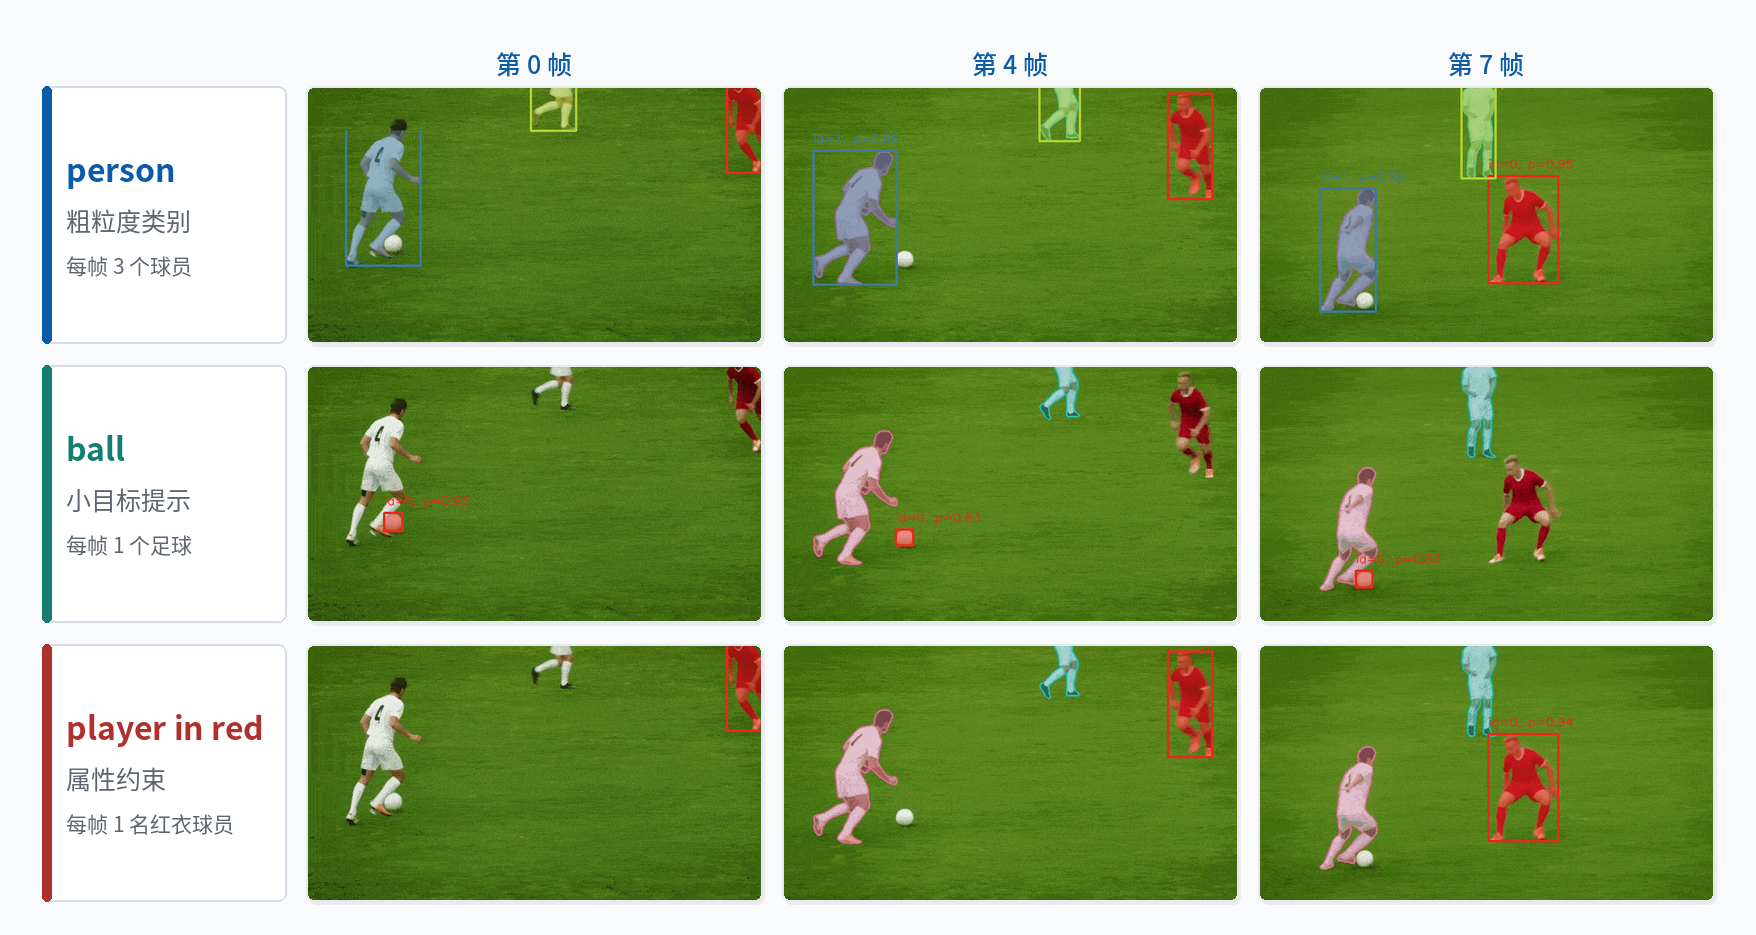
\includegraphics[width=0.98\textwidth]{sam31-video-prompt-grid.png}
  \caption{三组视频文本提示词的跨帧分割结果对比。每一行对应一个 prompt，每一列对应同一视频中的一个采样帧。}
  \label{fig:video-grid}
\end{figure}

\begin{lstlisting}[style=jsoncode,caption={\texttt{player in red} 实验 metadata 摘录}]
{
  "prompt": "player in red",
  "num_frames": 8,
  "selected_frames": [0, 4, 7],
  "load_seconds": 9.42,
  "inference_seconds": 1.49,
  "objects_per_frame": {
    "0": 1,
    "1": 1,
    "2": 1,
    "3": 1,
    "4": 1,
    "5": 1,
    "6": 1,
    "7": 1
  }
}
\end{lstlisting}

metadata 中记录了 prompt、采样帧、模型加载耗时、推理耗时和每帧目标数。以上耗时数据均由脚本自动记录至 metadata JSON 文件，随后整理为表格。

\subsection{粗粒度类别提示：person}

使用 \texttt{person} 提示时只给出人物类别，没有限制颜色或位置。模型将画面中符合人物概念的多个实例都找了出来，因此每帧得到 3 个目标。图~\ref{fig:video-grid} 第一行可以看到，白衣球员、红衣球员和远处球员被分配不同颜色和 id，目标集合在后续帧中保持稳定。

\subsection{小目标提示：ball}

足球面积小，和草地背景颜色也比较接近，属于这段视频中较难稳定跟踪的目标。使用 \texttt{ball} 提示时，模型仍能在每帧中保持 1 个足球目标输出。图~\ref{fig:video-grid} 第二行显示足球框会随运动位置更新，但 mask 面积较小，说明小目标结果对分辨率和置信度阈值更敏感。

\subsection{细粒度属性提示：player in red}

\texttt{player in red} 在类别基础上加入了颜色属性约束。与 \texttt{person} 不同，该提示并不要求输出全部人物，而是只锁定红色球衣球员。图~\ref{fig:video-grid} 第三行显示，模型每帧输出 1 个目标，并优先锁定红衣球员。这说明 SAM 3.1 的文本提示不仅能表达类别，也能表达颜色属性等细粒度概念。

\subsection{单帧图像补充实验}

为进一步验证模型在不同场景下的泛化能力，本实验补充选取校园夜景、车厢内日常物品场景和街景货车图片进行单帧开放词汇分割。图像实验共加载一次模型，加载时间为 6.12 s；每个 case 独立调用 \texttt{set\_image} 和 \texttt{set\_text\_prompt}。结果见表~\ref{tab:image-results} 和图~\ref{fig:image-grid}。

\begin{table}[H]
  \centering
  \footnotesize
  \setlength{\tabcolsep}{3pt}
  \caption{单帧图像文本提示实验结果}
  \label{tab:image-results}
  \begin{tabular}{L{2.0cm}L{1.8cm}L{1.3cm}L{1.4cm}L{1.3cm}L{4.3cm}}
    \toprule
    图像场景 & Prompt & 目标数 & 推理时间 & 最高分 & 观察结果 \\
    \midrule
    校园夜景 & \texttt{building} & 11 & 0.28 s & 0.859 & 能找出主楼和远处建筑，但夜景噪声使部分检测框较为零散。 \\
    校园夜景 & \texttt{tree} & 0 & 0.09 s & -- & 树木与暗背景区分度低，默认阈值下未保留实例。 \\
    车厢物品 & \texttt{bottle} & 0 & 0.09 s & -- & 目标被纸袋遮挡且外观不明显，未形成稳定候选。 \\
    街景货车 & \texttt{truck} & 1 & 0.09 s & 0.875 & 能完整覆盖整车主体。 \\
    街景货车 & \texttt{wheel} & 4 & 0.09 s & 0.949 & 能响应部件级提示，但也会包含车轮附近相似部件。 \\
    \bottomrule
  \end{tabular}
\end{table}

\begin{figure}[H]
  \centering
  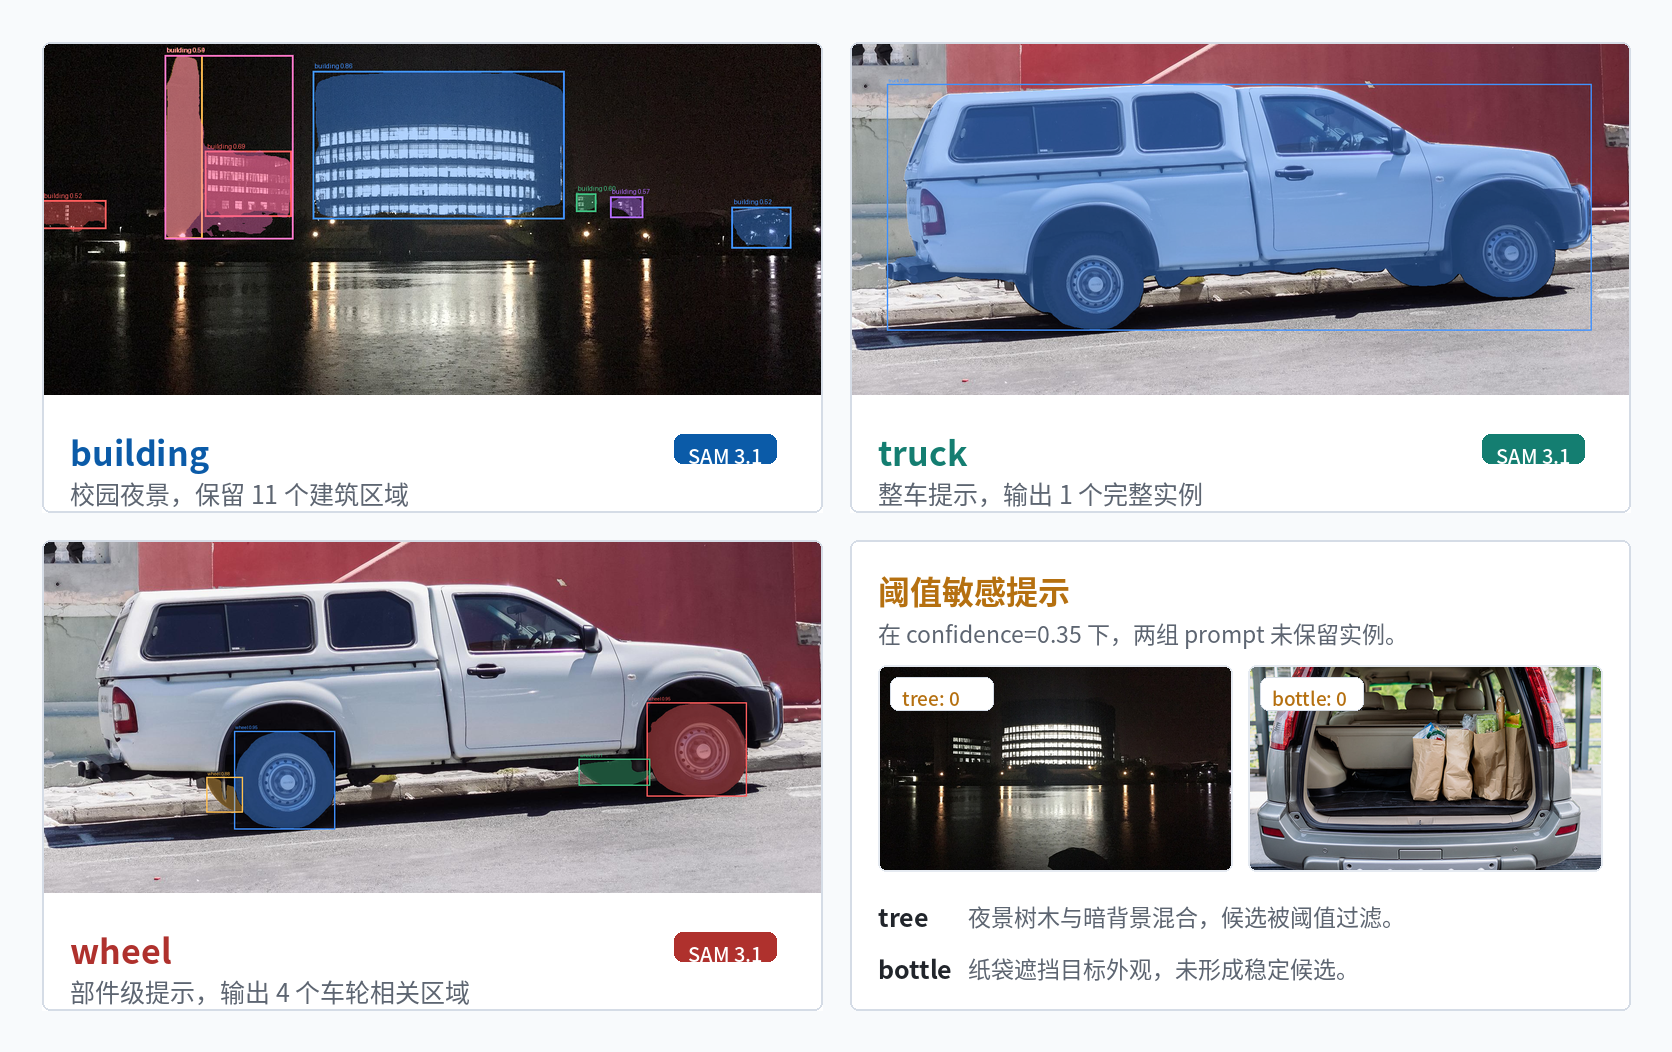
\includegraphics[width=0.98\textwidth]{sam31-image-cases-grid.png}
  \caption{单帧图像文本提示补充实验。成功样例覆盖场景级建筑、整车目标和车轮部件；右下角记录默认阈值下未保留实例的对照样例。}
  \label{fig:image-grid}
\end{figure}

\subsection{结果对比小结}

视频实验和单帧实验共同说明了 SAM 3.1 的开放词汇能力。类别提示更容易召回多个实例，例如 \texttt{person} 和 \texttt{building}；细粒度提示能将结果聚焦到特定目标，例如 \texttt{player in red} 和 \texttt{wheel}；小目标或遮挡目标更依赖图像清晰度和阈值设置，例如 \texttt{ball}、\texttt{tree} 和 \texttt{bottle}。因此，SAM 3.1 适合快速完成自然语言驱动的分割实验。如需进一步定量评测，可引入人工标注及 IoU、AP 等指标。

\section{问题处理与总结}

\subsection{运行中遇到的问题}

实验过程中主要处理了环境版本、依赖缺失、接口兼容和阈值选择四类问题。官方 README 推荐 CUDA 12.8 PyTorch，但本机驱动显示 CUDA 12.4，因此实际采用 \texttt{torch==2.6.0+cu124}。SAM3 源码导入 \texttt{pkg\_resources}，新版 setuptools 会导致模块缺失，所以固定 \texttt{setuptools<81}。此外，官方基础依赖没有完全覆盖 video predictor 的实际运行路径，需要额外安装 \texttt{einops}、\texttt{pycocotools}、\texttt{psutil} 等包。SAM3.1 multiplex 模型的 \texttt{init\_state} 参数签名与基类 \texttt{start\_session} 传入的参数不匹配，本实验脚本通过兼容启动函数规避了该问题，未改动官方源码。单帧图像实验中，\texttt{tree} 和 \texttt{bottle} 在默认阈值下没有输出，也说明开放词汇分割结果仍会受图像质量、遮挡和 confidence threshold 影响。

\subsection{实验结论}

本实验在本地 RTX 4090 上跑通了 SAM 3.1 的开放词汇视频分割、多目标跟踪和单帧图像提示分割。三组视频提示词分别验证了不同能力：\texttt{person} 对应多实例类别分割，\texttt{ball} 对应小目标定位，\texttt{player in red} 对应属性约束下的细粒度检索；单帧图像实验进一步展示了 \texttt{building}、\texttt{truck}、\texttt{wheel} 等不同粒度 prompt 的输出差异。从 PyTorch 源码角度来看，SAM 3.1 通过 \texttt{nn.Module} 组合、\texttt{state\_dict} 权重加载、\texttt{inference\_mode} 推理上下文、bf16/TF32 混合精度和 multiplex 矩阵映射，把 detector、tracker 和 memory encoder 等复杂模块封装在 session 请求接口后面；对外调用简洁，但内部数据流仍然是清晰的张量计算过程。

\subsection{后续改进}

后续可进一步增加自采视频或公开数据集样例，并比较 SAM 3、SAM 3.1 和 SAM 2.1 在相同视频上的速度与精度差异。单帧实验可以增加不同 confidence threshold 的扫描，观察召回率和误检之间的变化。如果环境支持 CUDA 12.8 和 FlashAttention 3，也可以重新开启 \texttt{use\_fa3} 与 \texttt{torch.compile}，评估 Object Multiplex 的实际加速效果。

\clearpage
\bibliographystyle{biblio/cumt-num}
\bibliography{biblio/references}

\end{document}
